\subsection{Datová vrstva IS}
Datová vrstva informačního systému \textbf{odděluje aplikaci od databáze}. Jde o třídy a funkce zajišťující komunikaci s databázi. \textbf{Překonává propast mezi SŘBD a programovacím jazykem}.

\begin{figure}[H]
	\centering
	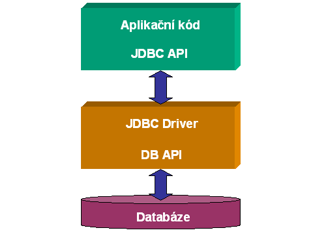
\includegraphics[width=0.48\textwidth]{assets/jdbc.png}
	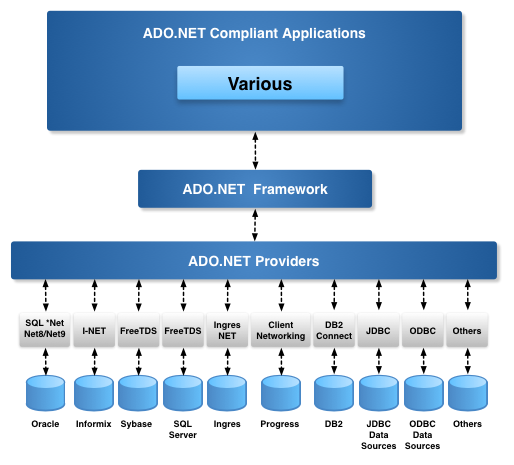
\includegraphics[width=0.4\textwidth]{assets/adonet.png}
\end{figure}

\begin{itemize}
\item \textbf{Nástroje} -- programovací jazyky + \textbf{SQL}, staví na \textbf{API pro dotazování DB} (JDBC, ADO.NET), \textbf{embedded SQL} - hostitelský jazyk obsahuje SQL.
\begin{itemize}
	\item \textbf{ODBC} (Open DataBase Conectivity) -- standartizované API pro přístup k databázovým systémům. ODBC se snaží poskytovat přístup nezávislý na programovacím jazyku, databazovem systému a operačním systému. 
	\item \textbf{JDBC} (Java DataBase Conectivity) -- Javovské API pro unifikovaný přístup k databazi. Bez ohledu kde jsou data uložena - SQL databáze, Oracle, XML, CSV, DB2, Ingress, ... -- se s nimi přes JDBC pracuje stejně.
	\item \textbf{ADO.NET} (Active Data Object) -- specifikace (knihovna) pro přísutupu k datový zdrojům na platformě .NET.
	\item \textbf{ASP.NET} -- knihovny pro informační systémy na platformě .NET. Pro komunikaci s databazi využívají ADO.NET.
	\item \textbf{Java2EE} -- knihovny pro informační systémy na platformě Java.
\end{itemize}
\item\textbf{Speciální prostředí} -- implementováno výrobcem SŘBD (Oracle Forms, APEX). Jednoduché, šité na míru, není připravené pro velké projekty a týmový vývoj.
\item \textbf{Architektury} -- jsou \textbf{komplikované}, \textbf{vícevrstvé}, ale umožňují jednodušší vývoj a zapojení více vývojářů. (3-vrstvá architektura => Business, Data, Presentation layer).
\end{itemize}

\subsubsection{JDBC}
\begin{itemize}
\item Rozhraní pro \textbf{unifikovaný přístup k datům} v DB na platformě \textbf{Java}.
\item Inspirováno rozhraním \textbf{ODBC}.
\item Zprostředkování komunikace aplikace s konkrétním typem DB (ovladače k většině).
\item \textbf{Dotazovací jazyk – SQL}. Předá se DB, ovladač vyhodnotí přímo.
\item \textbf{Schéma provedení dotazu:} 1) Připojení k datovému zdroji. 2) Inicializace. 3) Vytvoření a provedení dotazu. 4) Získání výsledku. 5) Ukončení transakce. 6) Odpojení od datového zdroje.
\item Hlavní třída \textbf{Connection} - odesílá \texttt{Statementy} a obdrží \texttt{ResultSety}.
\item \textbf{Podpora transakcí }(implicitně, každý příkaz jedna transakce, jsou vázány k instanci connection). 
\end{itemize}

\subsubsection{ADO.NET}
\begin{itemize}
\item \textbf{Connection} spouští \texttt{Commandy}, výsledkem je \texttt{DataSet} (použití \texttt{DataAdapteru}) nebo čistá data čtená \texttt{DataReaderem}.
\item \texttt{DataSet -> DataTable[] -> DataRow[] -> DataColumn[]}
\item \textbf{DataRelation} vazba mezi \texttt{DataSety} s vazebním \texttt{DataColumn}.
\item Umožňuje \textbf{parametrizovat commandy}.
\item Třída \textbf{\texttt{TransactionScope}} pro distribuované transakce.
\end{itemize}

\subsection{ORM (Objektově-relační mapování)}
Programovací technika \textbf{zpřístupňující relační či objektově-relační data pro objektové prostředí}. Entita v ORM je objekt, který je uložen v SŘBD (nejčastěji jako jeden záznam). Nejčastěji je implementován jako třída. Díky rozhraní jsou jednotlivé implementace zaměnitelné. Vlastnosti ORM rámců:
\begin{itemize} 
\item Práce s objektovým modelem (přenositelnost mezi různými SŘBD).
\item Překonává propast mezi SŘBD a programovacím jazykem.
\item \textbf{Rychlejší vytváření aplikací} vs Menší výkon aplikace.
\item Nevyužívá všechny vlastnosti SŘBD (efektivita, bezpečnost apod.).
\item Typová kontrola (nevznikají chyby v SQL).
\item Jednodušší testování.
\end{itemize}

\subsubsection{Pravidla ORM}
\begin{itemize}
\item \textbf{Minimalizace počtu dotazů }zasílaných na server.
\item \textbf{Minimalizovat objem dat} získaných z DB, stahovat pouze ta data, které potřebujeme, a které jsou zobrazeny uživateli (Lazy Loading).
\end{itemize}

\subsubsection{Vlastní implementace ORM}
\begin{itemize}
\item Využití \textbf{API pro komunikaci s DB} (JDBC, ADO.NET).
\item Používá se \textbf{SQL}.
\item \textbf{Výhody:} plná kontrola nad výkonem (stahujeme jen to co chceme) a prováděnými příkazy. Můžeme využít konkrétní prvky daného SŘBD.
\item \textbf{Nevýhody:} aplikace je závislá na určitém typu SŘBD.
\end{itemize}

\subsubsection{Automatizované}
\begin{itemize}
\item Frameworky \textbf{Hibernate} (Java), LINQ2SQL, \textbf{EntityFramework} (ASP.NET).
\item Může výrazně \textbf{degradovat výkon} (musí provádět interpretaci do SQL, vytváří objektový model atd.).
\item Většinou mají vlastní \textbf{cache}. Většinou jsou \textbf{nezávislé na daném SŘBD}.
\end{itemize}

\subsection{Bezpečnost}
\textbf{SQL Injection} - zranitelnost vznikající při nedostatečném \textbf{ošetření vstupů užívaných} v SQL dotazech. Např.: při přihlašování na webových stránkách zadá útoční příkaz SQL, které změní funkčnost dotazovaného příkazu. \textbf{Řešení:}
\begin{itemize}
\item \textbf{Parametrizované dotazy} (hodnoty jsou předány zvlášť, nemůže dojít k úpravě).
\item Uložené procedury.
\item Ošetření vstupů (\texttt{htmlspecialchars}, \texttt{mysql\_read\_escape\_string}) - zneužití např. pomocí jiného kódování!
\item Uživatel musí zadávat komplikovaná (neslovníková) hesla, \textbf{časové omezení počtu} pokusů. Logování neúspěšných pokusů o autentizaci.
\end{itemize}
